\clearpage

\renewcommand\thesection{\Alph{section}}

\setcounter{page}{1}
\setcounter{section}{0}
\maketitlesupplementary

A preview of SimBEV can be accessed at \href{https://gitfront.io/r/SportCarGallery/yY1YEo7uEcLB/SimBEV-Preview/}{https://gitfront .io/r/SportCarGallery/yY1YEo7uEcLB/SimBEV-Preview/}.

\section{CARLA Simulator}
\label{appsec:carla}

SimBEV relies on CARLA Simulator 0.9.15 \cite{dosovitskiy2017carla} equipped with an enhanced content library. Some of the improvements we made are listed below.
\begin{itemize}
    \item We added three new sports cars to CARLA's vehicle library using existing 3D models \cite{kentik2024mustang}\footnote{We used royalty-free 3D models of the three cars available on BlenderKit as the basis for the vehicles. However, the Supra and Chiron models had been removed from BlenderKit at the time of writing, so unfortunately we have no way of crediting their authors for their work.}: sixth generation Ford Mustang, Toyota GR Supra, and Bugatti Chiron, shown in \cref{appfig:car-trio}. They enhance the diversity of CARLA's vehicle library, especially when it comes to fast, high-performance cars. The Ford Mustang is the default data collection vehicle in SimBEV.
    \item We added lights (headlights, taillights, blinkers, etc.) to some of the older models in CARLA's vehicle library that lacked them, and redesigned existing vehicle lights in Blender using a new multi-layer approach that better visualizes modern multi-purpose lights, as shown in \cref{appfig:mustang-lights}.
    \item We added a set of 160 standard colors available to most vehicle models (apart from a few like the firetruck), and fixed color randomization issues for a few vehicles.
    \item We updated vehicle dynamics parameters of vehicle models to better match their vehicle's behavior and performance in the real world.
    \item We added or updated pedestrian navigation information for CARLA's Town12, Town13, and Town15 maps.
    \item We updated motorcycle and bicycle models so that they select their driver models randomly each time, instead of always being assigned the same model.
    \item We added lights to buildings in Town12 and fixed issues that prevented full control over building/street lights in Town12 and Town15.
\end{itemize}

SimBEV is compatible with the standard version of CARLA 0.9.15, but some features may not work properly.

\begin{figure}[t]
    \centering
    \setlength{\lineskip}{0pt}
    \includegraphics[width=\linewidth]{images/Trio5CR.png}
    \includegraphics[width=\linewidth]{images/Trio2CR.png}
    \caption{From left to right, the Bugatti Chiron, Ford Mustang, and Toyota GR Supra added to CARLA's vehicle library with their lights turned off (top) and on (bottom).}\label{appfig:car-trio}
\end{figure}
\begin{figure}[t]
    \centering
    \setlength{\belowcaptionskip}{-6 pt}
    \includegraphics[width=\linewidth]{images/MustangLights.png}
    \caption{In contrast to CARLA's segmented light design approach, our multi-layer approach can realistically visualize vehicle lights that use the same element for multiple purposes. For instance, in the Ford Mustang pictured here both position and left blinker lights are turned on.}\label{appfig:mustang-lights}
\end{figure}

\section{The SimBEV Dataset} \label{appsec:simbev-dataset-app}

\subsection{SimBEV configuration} \label{appsubsec:simbev-params}

We configured SimBEV to generate a diverse set of unique scenarios for the SimBEV dataset, and collected data from all sensor types supported by SimBEV (RGB, semantic segmentation, instance segmentation, depth, and optical flow cameras; regular and semantic lidar; radar; GNSS; and IMU). Sensor configurations are listed in \cref{apptable:sensor-properties} and the arrangement of the sensors on the ego vehicle is shown in \cref{appfig:sensor-fov} and \cref{appfig:sensor-coord}, and detailed in \cref{apptable:sensor-positions}.

\begin{table*}[t]
    \centering
    \footnotesize
    \begin{tabular}{l l}
        \toprule
        \textbf{Sensor type} & \textbf{Properties} \\
        \toprule
        RGB camera & 1600$\times$900 resolution, 80 deg FoV, $f/1.8$ \\
        All other cameras & 1600$\times$900 resolution, 80 deg FoV \\
        \multirow{2}*{Lidar} & 128 channels, 120.0 m range, 20.0 Hz rotation frequency, 5,242,880 points per second, -30.67 to 10.67 vertical FoV, \\
         & 14\% general drop-off rate, 1 cm radial noise std \\
        Semantic lidar & 128 channels, 120.0 m range, 20.0 Hz rotation frequency, 5,242,880 points per second, -30.67 to 10.67 vertical FoV \\
        Radar & 120.0 m range, 100 deg horizontal FoV, 12 deg vertical FoV, 40,000 points per second \\
        GNSS & \{4e-2 m, 4e-7 deg, 4e-7 deg\} noise std for \{altitude, latitude, longitude\} \\
        IMU & 1.7e-4 rad/s gyroscope bias, \{1.7e-4 m/s$^ {2}$, 5.6e-6 rad/s\} noise std for \{accelerometer, gyroscope\} \\
        \bottomrule
    \end{tabular}
    \caption{Sensor configurations used for the collection of the SimBEV dataset. std: standard deviation.} \label{apptable:sensor-properties}
\end{table*}
\begin{table}[t]
    \centering
    \footnotesize
    \setlength{\belowcaptionskip}{8 pt}
    \begin{tabular}{l c c c c}
        \toprule
        \textbf{Sensor} & \textbf{$x$ (m)} & \textbf{$y$ (m)}& \textbf{$z$ (m)} & \textbf{$\gamma$ (deg)} \\
        \toprule
        Front left camera & 0.4 & 0.4 & 1.6 & 55 \\
        Front camera & 0.6 & 0.0 & 1.6 & 0\\
        Front right camera & 0.4 & -0.4 & 1.6 & -55 \\
        Back left camera & 0.0 & 0.4 & 1.6 & 110 \\
        Back camera & -1.0 & 0.0 & 1.6 & 180 \\
        Back right camera & 0.0 & -0.4 & 1.6 & -110 \\
        Left radar & 0.0 & 1.0 & 0.6 & 90 \\
        Front radar & 2.4 & 0.0 & 0.6 & 0 \\
        Right radar & 0.0 & -1.0 & 0.6 & -90 \\
        Back radar & -2.4 & 0.0 & 0.6 & 180 \\
        Lidar & 0.0 & 0.0 & 1.8 & N/A \\
        \bottomrule
    \end{tabular}
    \caption{Arrangement of data collection sensors used in SimBEV and the SimBEV dataset. Coordinates are relative to the center of the ground plane of the ego vehicle's 3D bounding box.} \label{apptable:sensor-positions}
\end{table}
\begin{figure}[t]
    \centering
    \includegraphics[width=\linewidth]{figures/SensorFoV.pdf}
    \caption{Position and FoV of the perception sensors used in SimBEV to create the SimBEV dataset.}\label{appfig:sensor-fov}
\end{figure}

Our sensor setup was mostly inspired by \cite{caesar2020nuscenes} (e.g. the 1600$\times$900 image resolution, the arrangement of the cameras, and the lidar's vertical FoV), though there are a few differences. Our lidars (both regular and semantic) have 128 channels instead of 32 to collect a much denser point cloud, which can be downsampled by the user later on if desired. For GNSS and IMU, we used the bias and noise standard deviation values of a GNSS/INS module found in a typical experimental autonomous driving platform.

\begin{table}[t]
    \centering
    \footnotesize
    \setlength{\belowcaptionskip}{14 pt}
    \setlength{\tabcolsep}{4 pt}
    \begin{tabular}{l c l}
        \toprule
        \textbf{Parameter} & \textbf{Symbol} & \textbf{Distribution} \\
        \toprule
        Cloudiness & $k_{c}$ & $100\times\mathcal{B}(0.8, 1.0)$ \\
        Precipitation & $k_{p}$ & $\mathcal{B}(0.8, 0.2)\times k_{c}$ if $k_{c} > 40.0$ else 0.0 \\
        Precipitation & \multirow{2}*{$k_{pd}$} & \multirow{2}*{$k_{p} + \mathcal{B}(1.2, 1.6)\times(100 - k_{p})$} \\
        deposits \\
        Wetness & $k_{w}$ & $\min(100.0, \max(\mathcal{N}(k_{p}, 10.0)))$ \\
        Wind intensity & $k_{wi}$ & $\mathcal{U}(0.0, 100.0)$ \\
        Sun azimuth & \multirow{2}*{$k_{az}$} & \multirow{2}*{$\mathcal{U}(0.0, 360.0)$} \\
        angle \\
        Sun altitude & \multirow{2}*{$k_{al}$} & \multirow{2}*{$180\times\mathcal{B}(3.6, 2.0) - 90.0$} \\
        angle \\
        \multirow{2}*{Fog density} & \multirow{2}*{$k_{f}$} & $100\times\mathcal{B}(1.6, 2.0)$ if $k_{c} > 40.0$ \\
         &  & or $k_{al} < 10.0$ else 0.0 \\
        Fog distance & $k_{fd}$ & $\mathcal{LN}(3.2, 0.8)$ if $k_{f} > 10.0$ else 0.0 \\
        Fog falloff & $k_{ff}$ & $5.0\times\mathcal{B}(1.2, 2.4)$ if $k_{f} > 10.0$ else 1.0 \\
        \bottomrule
    \end{tabular}
    \caption{Probability distribution used in SimBEV for weather parameters. $\mathcal{B}$: beta distribution. $\mathcal{N}$: normal distribution. $\mathcal{U}$: uniform distribution. $\mathcal{LN}$: log-normal distribution.} \label{apptable:weather-distributions}
\end{table}

SimBEV uses the probability distributions listed in \cref{apptable:weather-distributions} to randomize the parameters that control the weather in CARLA. These distributions are interdependent to ensure that the resulting weather is realistic (e.g. a combination of heavy rain and clear sky is unrealistic). Each of the configured parameters is briefly discussed below.

\begin{figure}[t]
    \centering
    \includegraphics[width=\linewidth]{figures/SensorCoord.png}
    \caption{Coordinate frames of the perception sensors used in SimBEV to create the SimBEV dataset.}\label{appfig:sensor-coord}
\end{figure}
\begin{table*}[t]
    \centering
    \footnotesize
    \begin{tabular}{l c}
        \toprule
        \textbf{Parameter} & \textbf{Value or distribution} \\
        \toprule
        Warmup duration & 4 s \\
        Scene duration & 16 s \\
        Simulation time step & 50 ms \\
        3D bounding box collection radius & 120.0 m \\
        BEV grid resolution & $360\times360$ \\
        BEV grid cell dimensions & 0.4 m $\times$ 0.4 m \\
        Distance between CARLA-generated waypoints used for BEV ground truth calculation & 0.4 m \\
        Distance between CARLA-generated waypoints used as vehicle spawn location & 24.0 m \\
        Number of background vehicles ($s$: number of available spawn locations) & $\mathcal{U}_{i}(0, s - 3)$ \\
        Number of pedestrians & $\mathcal{U}_{i}(0, 640)$ \\
        Radius around the ego vehicle where background vehicles and pedestrians are spawned & 400.0 m \\
        Probability of vehicle door(s) getting open when stopped & 10.0\% \\
        Probability of emergency lights turned on & 50.0\% \\
        Probability of ego vehicle being reckless & 1.0\% \\
        Probability of other vehicles being reckless & 1.0\% \\
        Minimum speed of pedestrians & 0.8 m/s \\
        Maximum speed of pedestrians ($r$: minimum pedestrian speed) & $\max(r, \mathcal{LN}(0.16, 0.64))$ m/s \\
        Minimum intensity of street lights & 10,000 lm \\
        Change in the intensity of street lights ($m$: average intensity of all street lights in the scene) & $\mathcal{U}(-m, m)$ lm \\
        Probability of street light failure & 10.0\% \\
        Maximum vehicle speed relative to the speed limit & $\mathcal{U}(-20.0, 40.0)\%$ \\
        Distance to front vehicle when stopped & $\mathcal{N}(3.2, 1.0)$ m \\
        Traffic light green time & $\mathcal{U}(4.0, 28.0)$ s \\
        Walker cross factor & $\mathcal{B}(2.4, 1.6)$ \\
        \bottomrule
    \end{tabular}
    \caption{SimBEV configuration used for the collection of the SimBEV dataset. $\mathcal{B}$: beta distribution. $\mathcal{N}$: normal distribution. $\mathcal{U}$: uniform distribution. $\mathcal{U}_{i}$: uniform integer distribution. $\mathcal{LN}$: log-normal distribution.} \label{apptable:parameters}
\end{table*}
\begin{table}[t]
    \centering
    \footnotesize
    \setlength{\tabcolsep}{4 pt}
    \begin{tabular}{l c c c}
        \toprule
        \multirow{2}*{\textbf{Class}} & \textbf{Total 3D} & \textbf{Valid 3D}& \multirow{2}*{\textbf{BEV labes}} \\
         & \textbf{bounding boxes} & \textbf{bounding boxes} &  \\
        \toprule
        Road & N/A & N/A & 2,674,391,899 \\
        Car & 2,935,809 & 1,495,066 & 84,073,215 \\
        Truck & 497,729 & 298,280 & 22,759,787 \\
        Bus & 67,880 & 46,754 & 7,546,007 \\
        Motorcycle & 297,132 & 146,083 & 858,136 \\
        Bicycle & 214,619 & 100,640 & 187,869 \\
        Rider & N/A & N/A & 510,521 \\
        Pedestrian & 4,302,766 & 1,705,676 & 3,163,923 \\
        \toprule
        \textbf{Total} & 8,315,935 & 3,792,499 & 2,793,491,357 \\
        \bottomrule
    \end{tabular}
    \caption{Breakdown of the number of total and \textit{valid} 3D bounding boxes and BEV ground truth labels by class for the SimBEV dataset.} \label{apptable:overall-stats}
\end{table}

\begin{figure}[t]
    \centering
    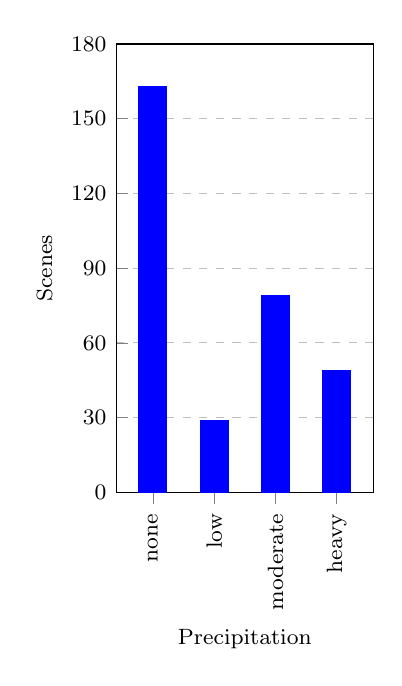
\begin{tikzpicture}
        \begin{axis}[title = {}, xlabel = {Precipitation}, xlabel near ticks, ylabel = {Scenes}, ylabel near ticks, xmin = 0.4, xmax = 4.6, ymin = 0, ymax = 180, ybar, xtick = {1, 2, 3, 4}, xticklabels = {none, low, moderate, heavy}, xticklabel style = {rotate = 90, anchor = east}, ytick = {0, 30, 60, 90, 120, 150, 180}, label style = {font = \footnotesize}, tick pos = left, tick label style = {font = \footnotesize}, ymajorgrids = true, grid style = dashed, width = 0.4\linewidth, height = 0.6\linewidth]
            \addplot[color = blue, fill = blue] coordinates {(1, 163) (2, 29) (3, 79) (4, 49)};
        \end{axis}
    \end{tikzpicture}
    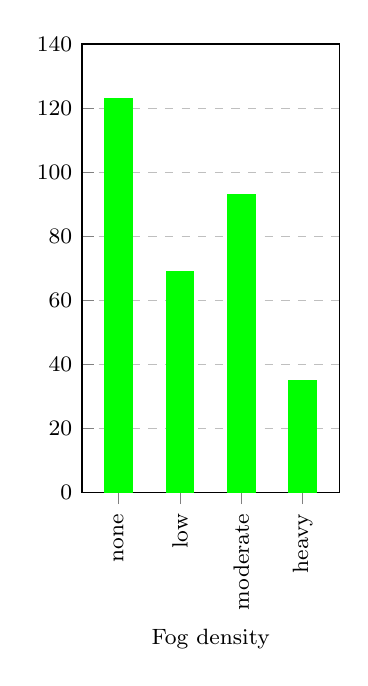
\begin{tikzpicture}
        \begin{axis}[title = {}, xlabel = {Fog density}, xlabel near ticks, xmin = 0.4, xmax = 4.6, ymin = 0, ymax = 140, ybar, xtick = {1, 2, 3, 4}, xticklabels = {none, low, moderate, heavy}, xticklabel style = {rotate = 90, anchor = east}, ytick = {0, 20, 40, 60, 80, 100, 120, 140}, label style = {font = \footnotesize}, tick pos = left, tick label style = {font = \footnotesize}, ymajorgrids = true, grid style = dashed, width = 0.4\linewidth, height = 0.6\linewidth]
            \addplot[color = green, fill = green] coordinates {(1, 123) (2, 69) (3, 93) (4, 35)};
        \end{axis}
    \end{tikzpicture}
    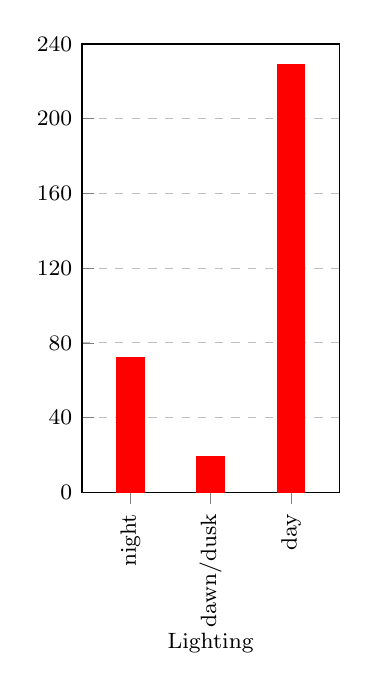
\begin{tikzpicture}
        \begin{axis}[title = {}, xlabel = {Lighting}, xlabel near ticks, xlabel shift = {-4.8 pt}, xmin = 0.4, xmax = 3.6, ymin = 0, ymax = 240, ybar, xtick = {1, 2, 3}, xticklabels = {night, dawn/dusk, day}, xticklabel style = {rotate = 90, anchor = east}, ytick = {0, 40, 80, 120, 160, 200, 240}, label style = {font = \footnotesize}, tick pos = left, tick label style = {font = \footnotesize}, ymajorgrids = true, grid style = dashed, width = 0.4\linewidth, height = 0.6\linewidth]
            \addplot[color = red, fill = red] coordinates {(1, 72) (2, 19) (3, 229)};
        \end{axis}
    \end{tikzpicture}
    \caption{Distribution of weather across SimBEV dataset scenes.} \label{appfig:weather-dist}
\end{figure}

\begin{itemize}
    \item Cloudiness ($k_{c}$) controls the volume of clouds. Values range from 0 to 100.
    \item Precipitation ($k_{p}$) controls the intensity of rain. Values range from 0 to 100.
    \item Precipitation deposits ($k_{pd}$) controls the amount of puddles. Values range from 0 to 100, with 0 being no puddles and 100 a road filled with water.
    \item Wetness ($k_{w}$) controls the intensity of camera image blurriness caused by rain. Values range from 0 to 100.
    \item Wind intensity ($k_{wi}$) controls the strength of wind. Values range from 0 to 100.
    \item Sun azimuth angle ($k_{az}$) controls the azimuth angle of the sun. Values range from 0 to 360.
    \item Sun altitude angle ($k_{al}$) controls the altitude angle of the sun. Values range from -90 to 90, with -90 representing midnight and 90 midday.
    \item Fog density ($k_{f}$) controls fog concentration or thickness. Values range from 0 to 100, with 0 being no fog.
    \item Fog distance ($k_{fd}$) controls how far away the fog starts, and can be any nonnegative number.
    \item Fog falloff ($k_{ff}$) controls the density of the fog (as in specific mass), and can be any nonnegative number. If set to 0, the fog will be lighter than air and will cover the whole scene. If set to 1, the fog is approximately as dense as air. For values greater than 5 the fog will be so dense that it will be compressed to the ground level. Fog falloff is set to 0.01 in Town12, Town13, and Town15 due to their non-zero elevation.
\end{itemize}
SimBEV leaves other weather parameters (such as scattering intensity and dust storm) at their default value, though the user can change them if desired.

\Cref{apptable:parameters} lists several other SimBEV configurations used to create the SimBEV dataset. They control various aspects of SimBEV such as scene duration, number of spawned background vehicles and pedestrians, driving behavior, chance of reckless driving, etc.

\subsection{SimBEV dataset statistics} \label{appsubsec:stats}

The SimBEV dataset comprises 102,400 annotated frames, 8,315,935 3D object bounding boxes (3,792,499 of which are \textit{valid}), and 2,793,491,357 BEV ground truth labels, broken down by class in \cref{apptable:overall-stats}. Cars and pedestrians make up the largest share of 3D object bounding boxes, though those boxes include a large number of motorcycles and bicycles as well. This makes sense since the majority of models in CARLA's vehicle library are cars (compared to, e.g., only one bus model). BEV labels are dominated by the \textit{road} class, followed by \textit{car}, \textit{truck}, and \textit{bus} due to their larger footprint compared to the rest.

As discussed previously, SimBEV randomizes CARLA's weather parameters according to the distributions specified in \cref{apptable:weather-distributions}. \Cref{appfig:weather-dist} shows the distribution of weather across the SimBEV dataset, where precipitation (rain intensity, $k_{p}$) and fog density ($k_{f}$) values for each scene are categorized into none ($<$10\%), low (10 - 40\%), moderate (40 - 70\%), and heavy (70 - 100\%); while sun altitude angle ($k_{al}$) is categorized into night (-90 - 0 deg), dawn/dusk (0 - 6 deg), and day (6 - 90 deg). \Cref{appfig:weather-dist} shows that SimBEV contains a good mix of different weather conditions, with rain or fog present in about half of the scenes and nearly a quarter of the scenes occurring at night.

Looking at the distribution of the number of spawned vehicles (cars, trucks, buses, motorcycles, bicycles) and pedestrians across scenes of the SimBEV dataset, shown in \cref{appfig:vehicle-ped-dist}, it is clear that the scenes range from relatively empty to congested and crowded. The distribution of pedestrians is supposed to be uniform, but CARLA often spawns fewer pedestrians than requested, and the number of unspawned pedestrians grows rapidly when hundreds of pedestrians are requested. Moreover, in some cases CARLA cannot spawn pedestrians because there are no walkable areas around the ego vehicle (e.g., when the ego vehicle is traveling on a rural road). Hence, there are many scenes with 0 and 240 - 320 pedestrians and very few with more than 480.

\begin{figure}[ht]
    \centering
    \setlength{\belowcaptionskip}{-4 pt}
    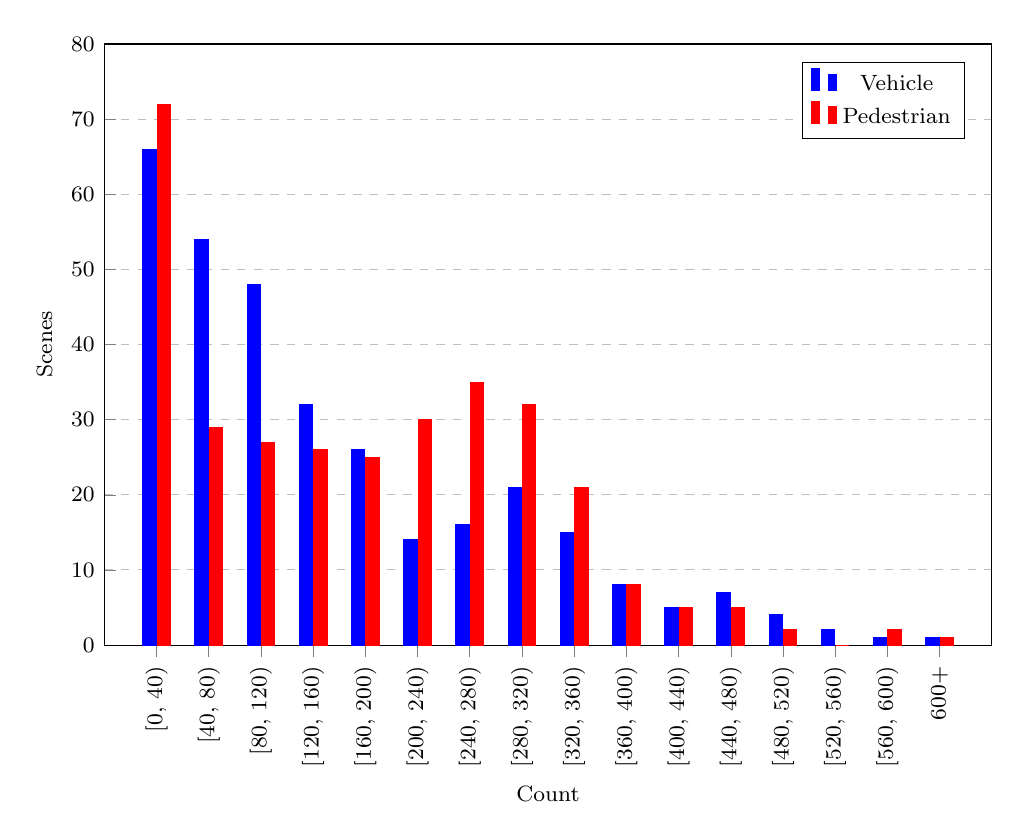
\begin{tikzpicture}
        \begin{axis}[title = {}, xlabel = {Count}, xlabel near ticks, ylabel = {Scenes}, ylabel near ticks, xmin = 0, xmax = 17, ymin = 0, ymax = 80, ybar = {0.4 pt}, bar width = {4.8 pt}, xtick = {1, 2, 3, 4, 5, 6, 7, 8, 9, 10, 11, 12, 13, 14, 15, 16}, xticklabels = {[0{,} 40), [40{,} 80), [80{,} 120), [120{,} 160), [160{,} 200), [200{,} 240), [240{,} 280), [280{,} 320), [320{,} 360), [360{,} 400), [400{,} 440), [440{,} 480), [480{,} 520), [520{,} 560), [560{,} 600), 600+}, xticklabel style = {rotate = 90, anchor = east}, ytick = {0, 10, 20, 30, 40, 50, 60, 70, 80}, label style = {font = \footnotesize}, tick pos = left, tick label style = {font = \footnotesize}, legend pos = north east, legend style = {font = \footnotesize}, ymajorgrids = true, grid style = dashed, width = 1.06\linewidth, height = 0.76\linewidth]
            \addplot[color = blue, fill = blue] coordinates {(1, 66) (2, 54) (3, 48) (4, 32) (5, 26) (6, 14) (7, 16) (8, 21) (9, 15) (10, 8) (11, 5) (12, 7) (13, 4) (14, 2) (15, 1) (16, 1)};
            \addplot[color = red, fill = red] coordinates {(1, 72) (2, 29) (3, 27) (4, 26) (5, 25) (6, 30) (7, 35) (8, 32) (9, 21) (10, 8) (11, 5) (12, 5) (13, 2) (14, 0) (15, 2) (16, 1)};
            \legend{Vehicle, Pedestrian}
        \end{axis}
    \end{tikzpicture}
    \caption{Distribution of the number of spawned vehicles (cars, trucks, buses, motorcycles, and bicycles) and pedestrians across the scenes of the SimBEV dataset.} \label{appfig:vehicle-ped-dist}
\end{figure}

\begin{figure}[ht]
    \centering
    \setlength{\belowcaptionskip}{-24 pt}
    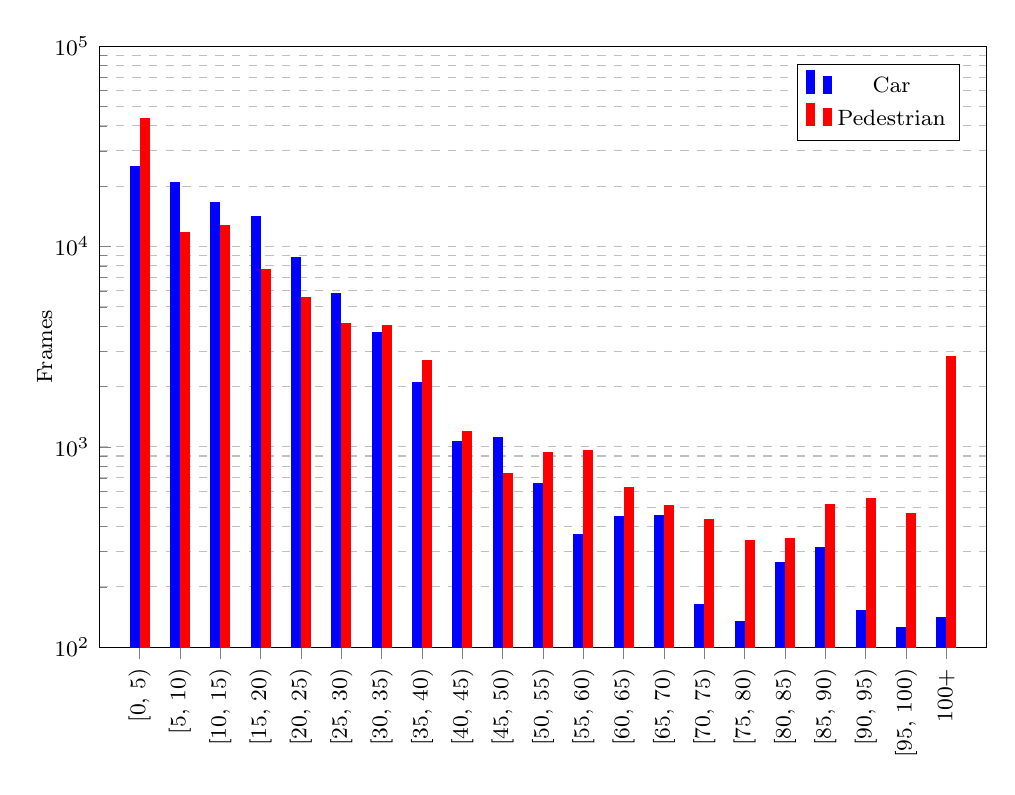
\begin{tikzpicture}
        \begin{semilogyaxis}[title = {}, xlabel near ticks, ylabel = {Frames}, ylabel near ticks, ylabel shift = {-6 pt}, xmin = 0, xmax = 22, ymin = 100, ymax = 100000, ybar = {0.4 pt}, bar width = {3.2 pt}, xtick = {1, 2, 3, 4, 5, 6, 7, 8, 9, 10, 11, 12, 13, 14, 15, 16, 17, 18, 19, 20, 21}, xticklabels = {[0{,} 5), [5{,} 10), [10{,} 15), [15{,} 20), [20{,} 25), [25{,} 30), [30{,} 35), [35{,} 40), [40{,} 45), [45{,} 50), [50{,} 55), [55{,} 60), [60{,} 65), [65{,} 70), [70{,} 75), [75{,} 80), [80{,} 85), [85{,} 90), [90{,} 95), [95{,} 100), 100+}, xticklabel style = {rotate = 90, anchor = east}, ytick = {100, 1000, 10000, 100000}, label style = {font = \footnotesize}, tick pos = left, tick label style = {font = \footnotesize}, legend pos = north east, legend style = {font = \footnotesize}, ymajorgrids = true, yminorgrids = true, grid style = dashed, width = 1.06\linewidth, height = 0.76\linewidth]
            \addplot[color = blue, fill = blue] coordinates {(1, 24985) (2, 20856) (3, 16656) (4, 14073) (5, 8809) (6, 5795) (7, 3728) (8, 2102) (9, 1062) (10, 1114) (11, 655) (12, 365) (13, 450) (14, 453) (15, 163) (16, 135) (17, 266) (18, 315) (19, 152) (20, 126) (21, 140)};
            \addplot[color = red, fill = red] coordinates {(1, 43457) (2, 11735) (3, 12716) (4, 7687) (5, 5534) (6, 4113) (7, 4035) (8, 2696) (9, 1194) (10, 735) (11, 938) (12, 959) (13, 623) (14, 509) (15, 435) (16, 341) (17, 347) (18, 515) (19, 552) (20, 467) (21, 2812)};
            \legend{Car, Pedestrian}
        \end{semilogyaxis}
    \end{tikzpicture}
    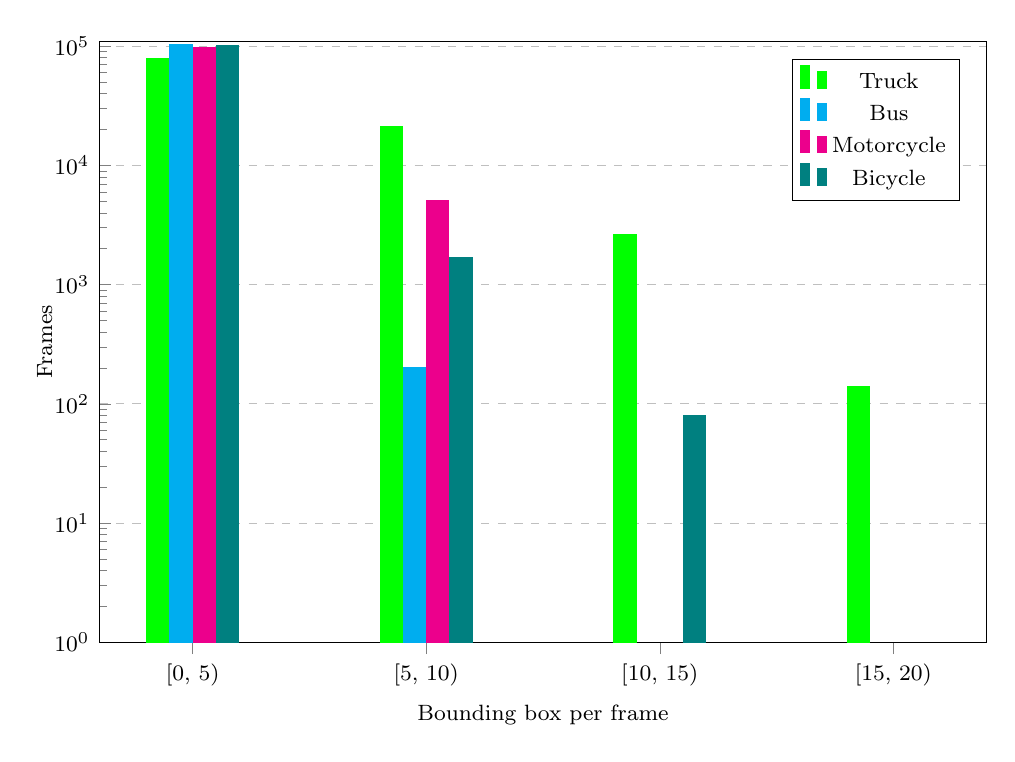
\begin{tikzpicture}
        \begin{semilogyaxis}[title = {}, xlabel = {Bounding box per frame}, xlabel near ticks, ylabel = {Frames}, ylabel near ticks, ylabel shift = {-6 pt}, xmin = 0.6, xmax = 4.4, ymin = 1, ymax = 110000, ybar = {0.4 pt}, bar width = {8 pt}, xtick = {1, 2, 3, 4}, xticklabels = {[0{,} 5), [5{,} 10), [10{,} 15), [15{,} 20)}, ytick = {1, 10, 100, 1000, 10000, 100000}, label style = {font = \footnotesize}, tick pos = left, tick label style = {font = \footnotesize}, legend pos = north east, legend style = {font = \footnotesize}, ymajorgrids = true, grid style = dashed, width = 1.06\linewidth, height = 0.76\linewidth]
            \addplot[color = green, fill = green] coordinates {(1, 78669) (2, 20969) (3, 2622) (4, 140)};
            \addplot[color = cyan, fill = cyan] coordinates {(1, 102200) (2, 200)};
            \addplot[color = magenta, fill = magenta] coordinates {(1, 97313) (2, 5087)};
            \addplot[color = teal, fill = teal] coordinates {(1, 100627) (2, 1693) (3, 80)};
            \legend{Truck, Bus, Motorcycle, Bicycle}
        \end{semilogyaxis}
    \end{tikzpicture}
    \caption{Breakdown of the number of \textit{valid} 3D object bounding boxes per frame by class across the SimBEV dataset.} \label{appfig:bbox-dist}
\end{figure}

\begin{figure}[ht]
    \centering
    \setlength{\belowcaptionskip}{-7.2 pt}
    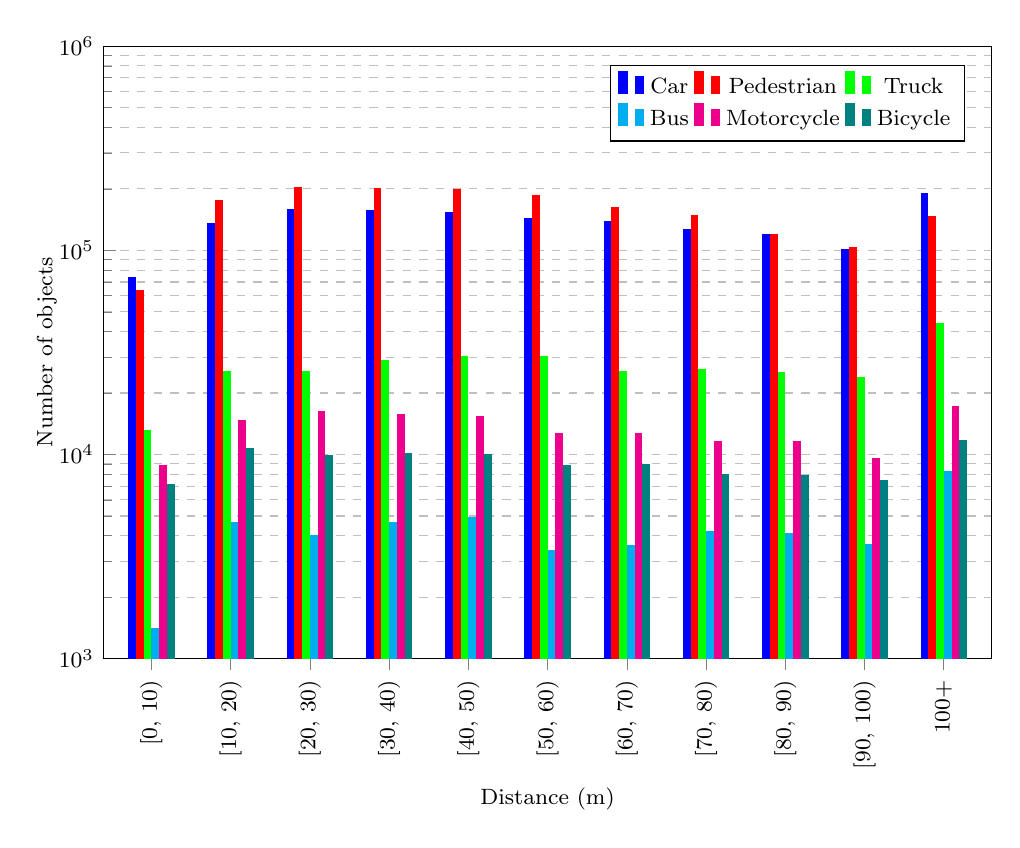
\begin{tikzpicture}
        \begin{semilogyaxis}[title = {}, xlabel = {Distance (m)}, xlabel near ticks, ylabel = {Number of objects}, ylabel near ticks, ylabel shift = {-6 pt}, xmin = 0.4, xmax = 11.6, ymin = 1000, ymax = 1000000, ybar = {0.4 pt}, bar width = {2.4 pt}, xtick = {1, 2, 3, 4, 5, 6, 7, 8, 9, 10, 11}, xticklabels = {[0{,} 10), [10{,} 20), [20{,} 30), [30{,} 40), [40{,} 50), [50{,} 60), [60{,} 70), [70{,} 80), [80{,} 90), [90{,} 100), 100+}, xticklabel style = {rotate = 90, anchor = east}, ytick = {1000, 10000, 100000, 1000000}, label style = {font = \footnotesize}, tick pos = left, tick label style = {font = \footnotesize}, legend pos = north east, legend style = {font = \footnotesize, legend columns = 3}, ymajorgrids = true, yminorgrids = true, grid style = dashed, width = 1.06\linewidth, height = 0.772\linewidth]
            \addplot[color = blue, fill = blue] coordinates {(1, 73296) (2, 135391) (3, 158103) (4, 156256) (5, 153405) (6, 143649) (7, 139089) (8, 125966) (9, 119928) (10, 100596) (11, 189387)};
            \addplot[color = red, fill = red] coordinates {(1, 63503) (2, 175807) (3, 203049) (4, 200182) (5, 197905) (6, 185989) (7, 162010) (8, 148013) (9, 119457) (10, 103498) (11, 146263)};
            \addplot[color = green, fill = green] coordinates {(1, 13125) (2, 25539) (3, 25460) (4, 28985) (5, 30271) (6, 30335) (7, 25506) (8, 26033) (9, 25300) (10, 23696) (11, 44030)};
            \addplot[color = cyan, fill = cyan] coordinates {(1, 1405) (2, 4626) (3, 4024) (4, 4632) (5, 4888) (6, 3382) (7, 3581) (8, 4208) (9, 4110) (10, 3627) (11, 8271)};
            \addplot[color = magenta, fill = magenta] coordinates {(1, 8835) (2, 14723) (3, 16277) (4, 15717) (5, 15315) (6, 12703) (7, 12630) (8, 11545) (9, 11589) (10, 9575) (11, 17174)};
            \addplot[color = teal, fill = teal] coordinates {(1, 7160) (2, 10714) (3, 9872) (4, 10118) (5, 10022) (6, 8869) (7, 8925) (8, 8011) (9, 7862) (10, 7420) (11, 11667)};
            \legend{Car, Pedestrian, Truck, Bus, Motorcycle, Bicycle}
        \end{semilogyaxis}
    \end{tikzpicture}
    \caption{Distribution of the distance of \textit{valid} objects from the ego vehicle across the SimBEV dataset.} \label{appfig:distance-dist}
\end{figure}

\begin{figure}[ht]
    \centering
    \setlength{\belowcaptionskip}{-24 pt}
    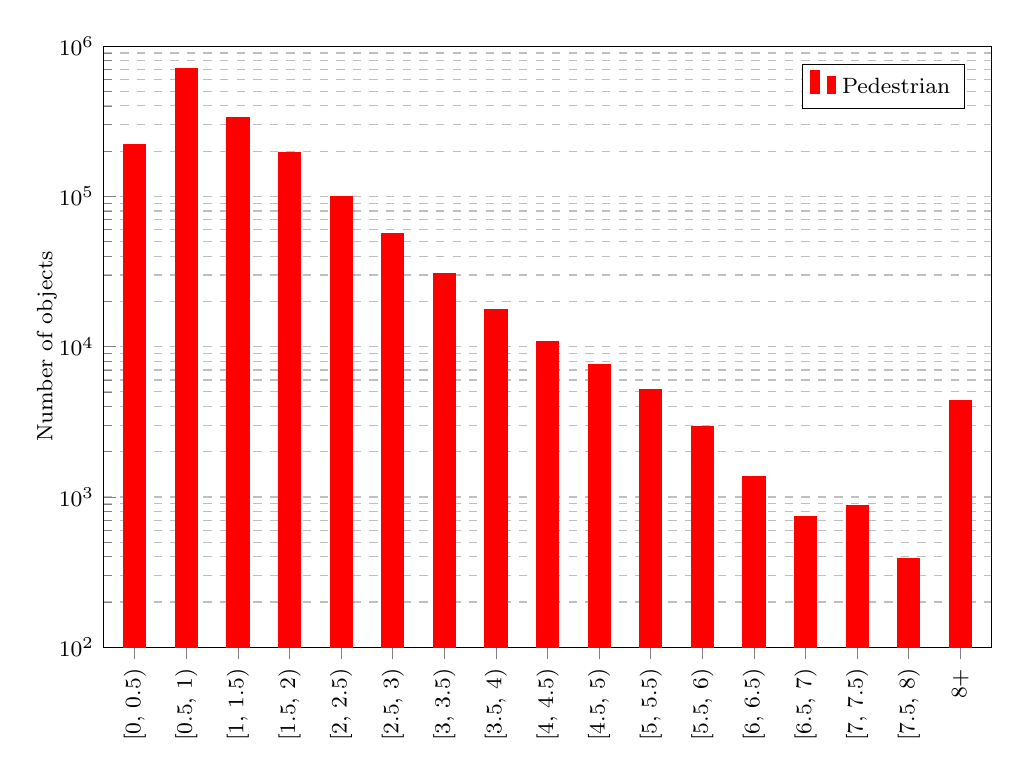
\begin{tikzpicture}
        \begin{semilogyaxis}[title = {}, xlabel near ticks, ylabel = {Number of objects}, ylabel near ticks, ylabel shift = {-6 pt}, xmin = 0.4, xmax = 17.6, ymin = 100, ymax = 1000000, ybar = {0.4 pt}, bar width = {8 pt}, xtick = {1, 2, 3, 4, 5, 6, 7, 8, 9, 10, 11, 12, 13, 14, 15, 16, 17}, xticklabels = {[0{,} 0.5), [0.5{,} 1), [1{,} 1.5), [1.5{,} 2), [2{,} 2.5), [2.5{,} 3), [3{,} 3.5), [3.5{,} 4), [4{,} 4.5), [4.5{,} 5), [5{,} 5.5), [5.5{,} 6), [6{,} 6.5), [6.5{,} 7), [7{,} 7.5), [7.5{,} 8), 8+}, xticklabel style = {rotate = 90, anchor = east}, ytick = {100, 1000, 10000, 100000, 1000000}, label style = {font = \footnotesize}, tick pos = left, tick label style = {font = \footnotesize}, legend pos = north east, legend style = {font = \footnotesize}, ymajorgrids = true, yminorgrids = true, grid style = dashed, width = 1.06\linewidth, height = 0.76\linewidth]
            \addplot[color = red, fill = red] coordinates {(1, 220987) (2, 711802) (3, 336667) (4, 196820) (5, 99965) (6, 56941) (7, 30475) (8, 17789) (9, 10792) (10, 7606) (11, 5147) (12, 2924) (13, 1370) (14, 741) (15, 871) (16, 390) (17, 4389)};
            \legend{Pedestrian}
        \end{semilogyaxis}
    \end{tikzpicture}
    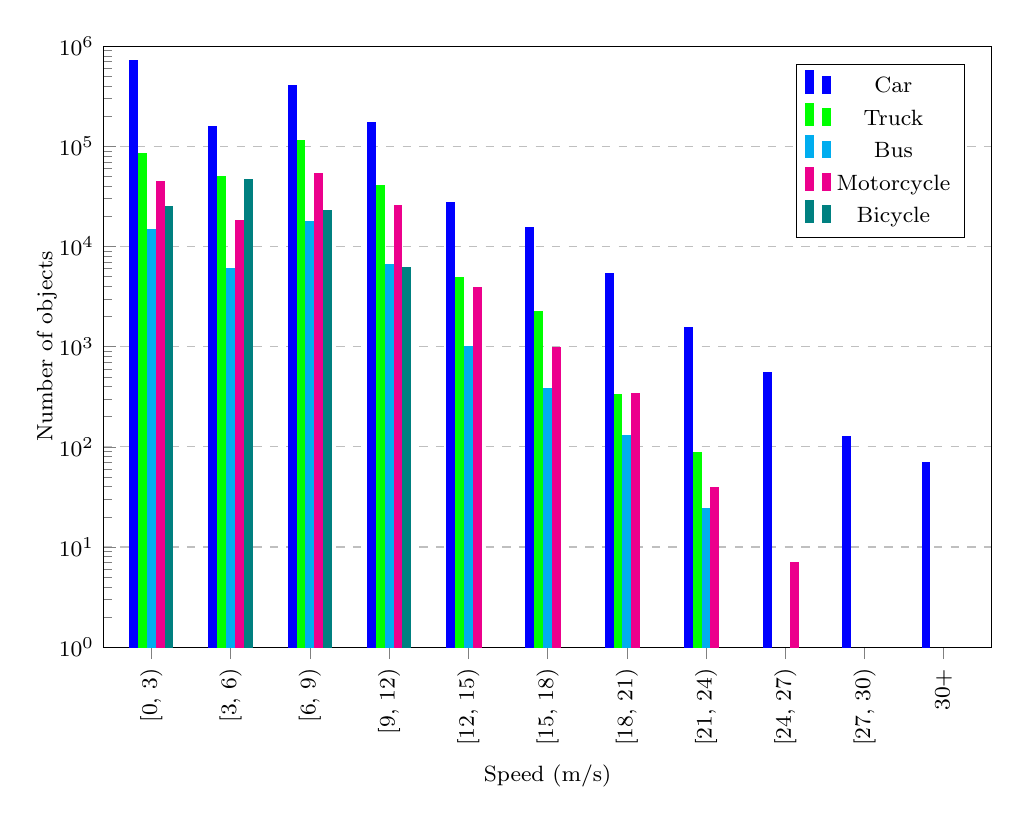
\begin{tikzpicture}
        \begin{semilogyaxis}[title = {}, xlabel = {Speed (m/s)}, xlabel near ticks, ylabel = {Number of objects}, ylabel near ticks, ylabel shift = {-6 pt}, xmin = 0.4, xmax = 11.6, ymin = 1, ymax = 1000000, ybar = {0.4 pt}, bar width = {2.8 pt}, xtick = {1, 2, 3, 4, 5, 6, 7, 8, 9, 10, 11}, xticklabels = {[0{,} 3), [3{,} 6), [6{,} 9), [9{,} 12), [12{,} 15), [15{,} 18), [18{,} 21), [21{,} 24), [24{,} 27), [27{,} 30), 30+}, xticklabel style = {rotate = 90, anchor = east}, ytick = {1, 10, 100, 1000, 10000, 100000, 1000000}, label style = {font = \footnotesize}, tick pos = left, tick label style = {font = \footnotesize}, legend pos = north east, legend style = {font = \footnotesize}, ymajorgrids = true, grid style = dashed, width = 1.06\linewidth, height = 0.76\linewidth]
            \addplot[color = blue, fill = blue] coordinates {(1, 712094) (2, 157149) (3, 402544) (4, 172628) (5, 27485) (6, 15449) (7, 5406) (8, 1558) (9, 557) (10, 126) (11, 70)};
            \addplot[color = green, fill = green] coordinates {(1, 85285) (2, 50492) (3, 113952) (4, 41052) (5, 4847) (6, 2230) (7, 334) (8, 88)};
            \addplot[color = cyan, fill = cyan] coordinates {(1, 14849) (2, 6005) (3, 17773) (4, 6588) (5, 1000) (6, 384) (7, 131) (8, 24)};
            \addplot[color = magenta, fill = magenta] coordinates {(1, 44343) (2, 17977) (3, 53109) (4, 25400) (5, 3895) (6, 970) (7, 343) (8, 39) (9, 7)};
            \addplot[color = teal, fill = teal] coordinates {(1, 25269) (2, 46072) (3, 23070) (4, 6229)};
            \legend{Car, Truck, Bus, Motorcycle, Bicycle}
        \end{semilogyaxis}
    \end{tikzpicture}
    \caption{Breakdown of the speed of \textit{valid} objects across the SimBEV dataset.} \label{appfig:velocity-dist}
\end{figure}



\begin{figure}[t]
    \centering
    \setlength{\belowcaptionskip}{-8 pt}
    \begin{tikzpicture}
        \begin{semilogyaxis}[title = {}, xlabel = {}, xlabel near ticks, ylabel = {Number of points}, ylabel near ticks, ylabel shift = {-6 pt}, xmin = 0, xmax = 120, ymin = 1, ymax = 100000, xtick = {}, xticklabel = {\empty}, ytick = {1, 10, 100, 1000, 10000, 100000}, label style = {font = \footnotesize}, tick pos = left, tick label style = {font = \footnotesize}, legend pos = north east, legend style = {font = \footnotesize, legend columns = 3}, width = 1.06\linewidth, height = \linewidth]
            \addlegendimage{only marks, color = blue}\addlegendentry{Car}
            \addlegendimage{only marks, color = red}\addlegendentry{Pedestrian}
            \addlegendimage{only marks, color = green}\addlegendentry{Truck}
            \addlegendimage{only marks, color = cyan}\addlegendentry{Bus}
            \addlegendimage{only marks, color = magenta}\addlegendentry{Motorcycle}
            \addlegendimage{only marks, color = teal}\addlegendentry{Bicycle}
            \addplot graphics[xmin = 0, xmax = 120, ymin = 1, ymax = 100000] {images/dist_num_lidar.png};
        \end{semilogyaxis}
    \end{tikzpicture}
    \begin{tikzpicture}
        \begin{semilogyaxis}[title = {}, xlabel = {Distance (m)}, xlabel near ticks, ylabel = {Number of points}, ylabel near ticks, ylabel shift = {-6 pt}, xmin = 0, xmax = 120, ymin = 1, ymax = 10000, xtick = {0, 20, 40, 60, 80, 100, 120}, ytick = {1, 10, 100, 1000, 10000}, label style = {font = \footnotesize}, tick pos = left, tick label style = {font = \footnotesize}, legend pos = north east, legend style = {font = \footnotesize, legend columns = 3}, width = 1.06\linewidth, height = \linewidth]
            \addlegendimage{only marks, color = blue}\addlegendentry{Car}
            \addlegendimage{only marks, color = red}\addlegendentry{Pedestrian}
            \addlegendimage{only marks, color = green}\addlegendentry{Truck}
            \addlegendimage{only marks, color = cyan}\addlegendentry{Bus}
            \addlegendimage{only marks, color = magenta}\addlegendentry{Motorcycle}
            \addlegendimage{only marks, color = teal}\addlegendentry{Bicycle}
            \addplot graphics[xmin = 0, xmax = 120, ymin = 1, ymax = 10000] {images/dist_num_radar.png};
        \end{semilogyaxis}
    \end{tikzpicture}
    \caption{Distribution of the number of lidar (top) and radar (bottom) points within \textit{valid} 3D object bounding boxes with respect to distance from the ego vehicle.} \label{appfig:num-points-dist}
\end{figure}

\begin{figure*}[t]
    \centering
    \begin{subfigure}{0.24\linewidth}
        \includegraphics[width=\linewidth]{images/log_label_0.png}
        \caption{Road} \label{subfig:road}
    \end{subfigure}
    \begin{subfigure}{0.24\linewidth}
        \includegraphics[width=\linewidth]{images/log_label_1.png}
        \caption{Car} \label{subfig:car}
    \end{subfigure}
    \begin{subfigure}{0.24\linewidth}
        \includegraphics[width=\linewidth]{images/log_label_2.png}
        \caption{Truck} \label{subfig:truck}
    \end{subfigure}
    \begin{subfigure}{0.24\linewidth}
        \includegraphics[width=\linewidth]{images/log_label_3.png}
        \caption{Bus} \label{subfig:bus}
    \end{subfigure}
    \begin{subfigure}{0.24\linewidth}
        \includegraphics[width=\linewidth]{images/log_label_4.png}
        \caption{Motorcycle} \label{subfig:motorcycle}
    \end{subfigure}
    \begin{subfigure}{0.24\linewidth}
        \includegraphics[width=\linewidth]{images/log_label_5.png}
        \caption{Bicycle} \label{subfig:bicycle}
    \end{subfigure}
    \begin{subfigure}{0.24\linewidth}
        \includegraphics[width=\linewidth]{images/log_label_6.png}
        \caption{Rider} \label{subfig:rider}
    \end{subfigure}
    \begin{subfigure}{0.24\linewidth}
        \includegraphics[width=\linewidth]{images/log_label_7.png}
        \caption{Pedestrian} \label{subfig:pedestrian}
    \end{subfigure}
    \setlength{\abovecaptionskip}{8 pt}
    \setlength{\belowcaptionskip}{-8 pt}
    \caption{Logarithmic BEV heat maps of the SimBEV dataset for different classes.} \label{appfig:bev-heat-map}
\end{figure*}

Because \cref{appfig:vehicle-ped-dist} shows the total number of spawned vehicles and pedestrians, many of which may be far from the ego vehicle, it may not fully represent what the ego vehicle observes. Hence in \cref{appfig:bbox-dist} we break down the number of \textit{valid} 3D object bounding boxes per frame by class. The distribution of the bounding boxes is similar to \cite{caesar2020nuscenes}, although our dataset offers a sizable number of frames with many (65+) \textit{valid} \textit{car}/\textit{pedestrian} bounding boxes as well. As expected, due to having fewer models in CARLA's vehicle library, the vast majority of frames only include a handful of trucks, buses, motorcycles, and bicycles.

\Cref{appfig:distance-dist} to \cref{appfig:num-points-dist} provide more insight into the SimBEV dataset. \Cref{appfig:distance-dist} shows that the distances of \textit{valid} 3D object bounding boxes from the ego vehicle are nearly uniformly distributed for all classes, in contrast to \cite{caesar2020nuscenes}, which is likely due to the higher density and range of our lidar point cloud. \Cref{appfig:velocity-dist} shows a reasonable speed range for all classes, which is comparable to \cite{caesar2020nuscenes} with a few exceptions. Our dataset has a large number of running pedestrians (3+ m/s), which can serve as edge cases for perception and behavior prediction algorithms. For other classes, our data was collected from both urban and highway environments (unlike \cite{caesar2020nuscenes}, which only collected data from urban environments), leading to many fast-moving objects. \cref{appfig:num-points-dist} shows the distribution of the number of lidar and radar points within \textit{valid} 3D object bounding boxes with respect to distance from the ego vehicle. Consistent with \cite{caesar2020nuscenes}, larger object bounding boxes have more points inside and the number of points for all classes decreases with increasing distance.

Finally, logarithmic BEV ground truth heat maps for all classes of the SimBEV dataset are shown in \cref{appfig:bev-heat-map}. As expected, \textit{road} is concentrated in the direction of travel of the ego vehicle, which also results in the concentration of labels of all vehicular classes in that region. In contrast, \textit{pedestrian} labels are relatively evenly distributed.

\section{3D Object Detection Evaluation}

For both approaches to evaluating the results of 3D object detection, AP is calculated from the area under the precision-recall curve. For the first method, we use IoU thresholds of $\mathbb{T} = \{0.3, 0.4, 0.5, 0.6, 0.7, 0.8, 0.9\}$ to match the bounding boxes. For the second method, similar to \cite{caesar2020nuscenes}, we use distance thresholds of $\mathbb{T} = \{0.5, 1, 2, 4\}$ m to match the bounding boxes. For both approaches, we define mAP as the average over all classes and all matching thresholds:
\begin{equation} \label{eq:map}
    \mathrm{mAP} = \frac{1}{|\mathbb{T}||\mathbb{C}|}\sum_{t \in \mathbb{T}, c \in \mathbb{C}}\mathrm{AP}_{t, c}.
\end{equation}

Similar to \cite{caesar2020nuscenes}, we measure a set of True Positive metrics (TP metrics) for each predicted bounding box that is matched to a ground truth bounding box: Average Translation Error (ATE), which is the Euclidean distance (in m) between box centers; Average Orientation Error (AOE), which is the smallest yaw angle difference (in rad) between the two boxes; Average Scale Error (ASE), which is equal to one minus the 3D IoU value of the two boxes after aligning for orientation and translation; and Average Velocity Error (AVE), which is the L2 norm of the difference in box velocities (in m/s). The mean TP metric (mTP) for each metric is computed by averaging over all classes and thresholds:
\begin{equation} \label{eq:mtp}
    \mathrm{mTP} = \frac{1}{|\mathbb{T}||\mathbb{C}|}\sum_{t \in \mathbb{T}, c \in \mathbb{C}}\mathrm{TP}_{t, c}.
\end{equation}

Finally, similar to \cite{caesar2020nuscenes}, we define the SimBEV Detection Score (SDS) as:
\begin{equation} \label{eq:sds}
    \mathrm{SDS} = \frac{1}{8}\Big(4\,\mathrm{mAP} + \sum_{\mathrm{mTP} \in \mathbb{TP}}(1-\min(1, \mathrm{mTP}))\Big).
\end{equation}

\section{Model Implementation} \label{appsec:model-implementation}

All variants of BEVFusion \cite{liu2022bevfusion} and UniTR \cite{wang2023unitr} were trained on an Nvidia DGX A100 640GB node using the settings and hyperparameters used by their authors for benchmarking on the nuScenes dataset \cite{caesar2020nuscenes}. SimBEV dataset data were augmented (translated, rotated, scaled) during training for all models.

\section{Comprehensive Evaluation Results} \label{appsec:comp-eval-results}

\begin{table*}[ht]
    \centering
    \footnotesize
    % \setlength{\tabcolsep}{2.4 pt}
    % \setlength{\belowcaptionskip}{-24 pt}
    \begin{tabular}{l c c c c c c c c c c c}
        \toprule
        \textbf{Class} & \textbf{Model} & \textbf{Modality} & \textbf{0.1} & \textbf{0.2} & \textbf{0.3} & \textbf{0.4} & \textbf{0.5} & \textbf{0.6} & \textbf{0.7} & \textbf{0.8} & \textbf{0.9} \\
        \toprule
        \multirow{5}*{Road} & BEVFusion-C & C & 59.5 & 67.1 & 71.5 & 74.5 & 76.0 & 75.2 & 72.6 & 68.9 & 62.3 \\
         & BEVFusion-L & L & 48.6 & 55.9 & 66.1 & 85.1 & 87.7 & 87.2 & 84.9 & 81.1 & 74.6 \\
         & BEVFusion & C + L & \bb{59.7} & \bb{72.0} & \bb{80.0} & \bb{85.5} & \bb{88.4} & \bb{88.1} & \bb{85.9} & \bb{82.4} & \bb{76.3} \\
         & UniTR & C + L & \gb{85.7} & \gb{89.1} & \gb{91.0} & \gb{92.2} & \gb{92.8} & \gb{92.5} & \gb{91.4} & \gb{89.3} & \gb{85.5} \\
         & UniTR+LSS & C + L & \rb{86.0} & \rb{89.4} & \rb{91.3} & \rb{92.6} & \rb{93.3} & \rb{93.0} & \rb{92.0} & \rb{90.1} & \rb{86.4} \\
        \midrule
        \multirow{5}*{Car} & BEVFusion-C & C & 3.5 & 8.0 & 18.8 & 22.4 & 17.2 & 11.3 & 9.7 & 8.7 & 6.3 \\
         & BEVFusion-L & L & 5.3 & 37.8 & 56.5 & 67.1 & 70.6 & 63.6 & 51.8 & 37.6 & 18.8 \\
         & BEVFusion & C + L & \bb{11.7} & \bb{39.4} & \bb{58.6} & \bb{69.4} & \bb{72.7} & \bb{65.5} & \bb{54.0} & \bb{40.1} & \bb{20.5} \\
         & UniTR & C + L & \gb{31.2} & \gb{49.6} & \rb{63.1} & \rb{71.3} & \rb{73.8} & \rb{67.4} & \rb{57.4} & \rb{45.8} & \rb{29.8} \\
         & UniTR+LSS & C + L & \rb{32.2} & \rb{50.6} & \gb{63.0} & \gb{70.9} & \gb{72.8} & \gb{66.1} & \gb{55.8} & \gb{44.3} & \gb{28.8} \\
        \midrule
        \multirow{5}*{Truck} & BEVFusion-C & C & 2.1 & 6.7 & 11.7 & 9.8 & 5.1 & 2.1 & 0.4 & 0.0 & 0.0 \\
         & BEVFusion-L & L & 11.4 & 44.7 & 61.2 & \gb{70.6} & \gb{73.5} & \gb{67.4} & \gb{55.2} & 39.5 & 16.3 \\
         & BEVFusion & C + L & \bb{12.3} & \bb{47.0} & \bb{61.4} & \rb{70.9} & \rb{74.5} & \rb{69.2} & \rb{57.6} & \rb{43.2} & \bb{20.6} \\
         & UniTR & C + L & \gb{33.3} & \gb{51.2} & \gb{61.7} & 67.2 & 67.7 & 61.3 & 51.9 & \bb{40.1} & \gb{22.7} \\
         & UniTR+LSS & C + L & \rb{34.4} & \rb{53.2} & \rb{63.6} & \bb{69.0} & \bb{69.4} & \bb{63.4} & \bb{53.6} & \gb{41.6} & \rb{23.6} \\
        \midrule
        \multirow{5}*{Bus} & BEVFusion-C & C & 2.1 & 9.0 & 19.9 & 24.6 & 22.9 & 16.8 & 10.3 & 6.0 & 1.1 \\
         & BEVFusion-L & L & 19.1 & \gb{56.9} & \rb{72.0} & \rb{79.7} & \rb{81.5} & \rb{78.1} & \rb{69.7} & \rb{59.4} & \rb{44.1} \\
         & BEVFusion & C + L & \bb{19.7} & \bb{56.8} & \gb{70.3} & \gb{78.2} & \gb{80.8} & \gb{77.2} & \gb{68.9} & \gb{59.0} & \rb{44.1} \\
         & UniTR & C + L & \gb{39.5} & 53.5 & 56.7 & 55.5 & 51.7 & 45.1 & 37.8 & 29.8 & \bb{17.9} \\
         & UniTR+LSS & C + L & \rb{44.4} & \rb{57.2} & \bb{61.7} & \bb{62.0} & \bb{58.5} & \bb{51.4} & \bb{42.9} & \bb{33.5} & \gb{21.3} \\
        \midrule
        \multirow{5}*{Motorcycle} & BEVFusion-C & C & 0.3 & 0.7 & 0.0 & 0.0 & 0.0 & 0.0 & 0.0 & 0.0 & 0.0 \\
         & BEVFusion-L & L & 4.8 & \bb{13.7} & \gb{23.6} & 32.7 & 32.5 & 15.8 & 0.8 & 0.0 & 0.0 \\
         & BEVFusion & C + L & \bb{5.0} & 13.5 & \gb{23.6} & \bb{34.6} & \gb{36.3} & \bb{18.3} & \bb{1.5} & 0.0 & 0.0 \\
         & UniTR & C + L & \gb{6.2} & \gb{17.6} & \rb{29.1} & \rb{37.4} & \rb{36.5} & \rb{22.7} & \rb{7.2} & \rb{0.3} & 0.0 \\
         & UniTR+LSS & C + L & \rb{8.3} & \rb{19.5} & \rb{29.1} & \gb{36.3} & \bb{35.9} & \gb{21.6} & \gb{5.8} & \rb{0.3} & 0.0 \\
        \midrule
        \multirow{5}*{Bicycle} & BEVFusion-C & C & 0.0 & 0.0 & 0.0 & 0.0 & 0.0 & 0.0 & 0.0 & 0.0 & 0.0 \\
         & BEVFusion-L & L & 1.8 & 5.1 & 10.0 & \gb{13.3} & \bb{3.6} & 0.0 & 0.0 & 0.0 & 0.0 \\
         & BEVFusion & C + L & \bb{1.9} & \bb{5.6} & \rb{11.1} & \bb{12.7} & \bb{3.6} & 0.0 & 0.0 & 0.0 & 0.0 \\
         & UniTR & C + L & \rb{3.3} & \rb{7.9} & \gb{11.0} & \rb{13.6} & \rb{11.4} & \rb{5.5} & \gb{0.7} & 0.0 & 0.0 \\
         & UniTR+LSS & C + L & \gb{3.2} & \gb{7.7} & \bb{10.5} & 10.9 & \gb{6.3} & \gb{2.7} & \rb{1.4} & \rb{0.2} & 0.0 \\
        \midrule
        \multirow{5}*{Rider} & BEVFusion-C & C & 0.3 & 0.1 & 0.0 & 0.0 & 0.0 & 0.0 & 0.0 & 0.0 & 0.0 \\
         & BEVFusion-L & L & 4.6 & 11.7 & 20.8 & 30.3 & 18.4 & 0.5 & 0.0 & 0.0 & 0.0 \\
         & BEVFusion & C + L & \bb{4.8} & \bb{11.9} & \bb{21.0} & \bb{31.0} & \bb{23.3} & \bb{1.2} & 0.0 & 0.0 & 0.0 \\
         & UniTR & C + L & \gb{5.3} & \gb{15.5} & \rb{25.7} & \rb{35.7} & \rb{36.2} & \rb{17.4} & \rb{1.7} & 0.0 & 0.0 \\
         & UniTR+LSS & C + L & \rb{6.5} & \rb{15.7} & \gb{24.4} & \gb{32.1} & \gb{31.6} & \gb{14.8} & \gb{1.3} & 0.0 & 0.0 \\
        \midrule
        \multirow{5}*{Pedestrian} & BEVFusion-C & C & \bb{0.2} & 0.0 & 0.0 & 0.0 & 0.0 & 0.0 & 0.0 & 0.0 & 0.0 \\
         & BEVFusion-L & L & \rb{3.1} & 9.6 & 17.6 & \bb{28.4} & \bb{18.9} & \bb{0.1} & 0.0 & 0.0 & 0.0 \\
         & BEVFusion & C + L & \rb{3.1} & \bb{9.9} & \gb{18.3} & \gb{28.7} & \gb{20.2} & \gb{0.2} & 0.0 & 0.0 & 0.0 \\
         & UniTR & C + L & \gb{3.0} & \rb{11.1} & \rb{19.9} & \rb{30.2} & \rb{27.5} & \rb{3.9} & 0.0 & 0.0 & 0.0 \\
         & UniTR+LSS & C + L & \rb{3.1} & \gb{10.2} & \bb{17.7} & 25.1 & 12.9 & \gb{0.2} & 0.0 & 0.0 & 0.0 \\
        \midrule
        \midrule
        \multirow{5}*{Mean} & BEVFusion-C & C & 8.5 & 11.4 & 15.2 & 16.4 & 15.2 & 13.2 & 11.6 & 10.5 & 8.7 \\
         & BEVFusion-L & L & 12.4 & 29.4 & 41.0 & \gb{50.9} & \bb{48.3} & \bb{39.1} & \gb{32.8} & \gb{27.2} & 19.2 \\
         & BEVFusion & C + L & \bb{14.8} & \bb{32.0} & \bb{43.0} & \rb{51.3} & \rb{50.0} & \rb{40.0} & \rb{33.5} & \rb{28.1} & \rb{20.2} \\
         & UniTR & C + L & \gb{25.9} & \gb{36.9} & \gb{44.8} & \bb{50.4} & \gb{49.7} & \gb{39.5} & 31.0 & 25.7 & \bb{19.5} \\
         & UniTR+LSS & C + L & \rb{27.3} & \rb{38.0} & \rb{45.2} & 49.9 & 47.6 & \bb{39.1} & \bb{31.6} & \bb{26.2} & \gb{20.0} \\
        \bottomrule
    \end{tabular}
    \caption{BEV segmentation IoUs (in \%) by class and IoU threshold for different models evaluated on the SimBEV dataset \textit{test} set. The top three values are indicated in \rb{red}, \gb{green}, and \bb{blue}, respectively.} \label{apptable:comp-seg}
\end{table*}
\begin{table*}[ht]
    \centering
    \footnotesize
    % \setlength{\tabcolsep}{4pt}
    \begin{tabular}{l c c c c c c c}
        \toprule
        \multirow{2}*{\textbf{Class}} & \multirow{2}*{\textbf{Model}} & \multirow{2}*{\textbf{Modality}} & \textbf{mAP} & \textbf{mATE} & \textbf{mAOE} & \textbf{mASE} & \textbf{mAVE} \\
         & & & \textbf{(\%) $\uparrow$} & \textbf{(m) $\downarrow$} & \textbf{(rad) $\downarrow$} & \textbf{$\downarrow$} & \textbf{(m/s) $\downarrow$} \\
        \toprule
        \multirow{5}*{Car} & BEVFusion-C & C & 12.5 & 0.518 & 0.710 & 0.177 & 5.67 \\
         & BEVFusion-L & L & \gb{41.0} & 0.129 & \gb{0.080} & 0.113 & 1.40 \\
         & BEVFusion & C + L & \rb{41.1} & \bb{0.128} & \rb{0.078} & \bb{0.112} & \bb{1.37} \\
         & UniTR & C + L & 38.8 & \gb{0.100} & 0.123 & \rb{0.084} & \gb{0.49} \\
         & UniTR+LSS & C + L & \bb{39.8} & \rb{0.099} & \bb{0.106} & \gb{0.087} & \rb{0.47} \\
        \midrule
        \multirow{5}*{Truck} & BEVFusion-C & C & 14.1 & 0.568 & 0.902 & 0.123 & 6.64 \\
         & BEVFusion-L & L & \rb{38.7} & \bb{0.143} & \rb{0.040} & 0.100 & 1.73 \\
         & BEVFusion & C + L & \rb{38.7} & 0.149 & \gb{0.042} & \bb{0.096} & \bb{1.70} \\
         & UniTR & C + L & \bb{36.2} & \rb{0.108} & 0.098 & \rb{0.066} & \gb{0.56} \\
         & UniTR+LSS & C + L & \gb{36.6} & \gb{0.110} & \bb{0.096} & \gb{0.070} & \rb{0.55} \\
        \midrule
        \multirow{5}*{Bus} & BEVFusion-C & C & 17.4 & 0.967 & 1.225 & \rb{0.020} & 5.80 \\
         & BEVFusion-L & L & \rb{30.6} & \bb{0.159} & \gb{0.044} & 0.067 & \bb{2.32} \\
         & BEVFusion & C + L & \gb{30.5} & 0.164 & \rb{0.037} & 0.058 & 2.42 \\
         & UniTR & C + L & 25.6 & \rb{0.114} & 0.143 & \bb{0.038} & \gb{0.85} \\
         & UniTR+LSS & C + L & \bb{27.4} & \gb{0.124} & \bb{0.121} & \gb{0.036} & \rb{0.75} \\
        \midrule
        \multirow{5}*{Motorcycle} & BEVFusion-C & C & 11.6 & 0.261 & 0.688 & 0.135 & 6.63 \\
         & BEVFusion-L & L & 39.6 & \gb{0.091} & \gb{0.080} & 0.131 & 1.74 \\
         & BEVFusion & C + L & \gb{40.1} & \bb{0.092} & \rb{0.071} & \bb{0.125} & \bb{1.59} \\
         & UniTR & C + L & \bb{39.8} & \rb{0.074} & 0.102 & \gb{0.092} & \rb{0.54} \\
         & UniTR+LSS & C + L & \rb{40.4} & \rb{0.074} & \bb{0.097} & \rb{0.088} & \gb{0.56} \\
        \midrule
        \multirow{5}*{Bicycle} & BEVFusion-C & C & 8.4 & 0.227 & 0.818 & 0.200 & 3.20 \\
         & BEVFusion-L & L & \bb{38.4} & \bb{0.088} & \gb{0.071} & 0.186 & 1.46 \\
         & BEVFusion & C + L & 38.3 & 0.089 & \rb{0.054} & \bb{0.177} & \bb{1.41} \\
         & UniTR & C + L & \gb{39.5} & \gb{0.071} & 0.110 & \gb{0.120} & \rb{0.43} \\
         & UniTR+LSS & C + L & \rb{41.3} & \rb{0.069} & \bb{0.103} & \rb{0.103} & \gb{0.44} \\
        \midrule
        \multirow{5}*{Pedestrian} & BEVFusion-C & C & 0.2 & 0.111 & 1.42 & \rb{0.035} & 1.18 \\
         & BEVFusion-L & L & 37.0 & \bb{0.064} & \gb{0.262} & 0.076 & \bb{0.39} \\
         & BEVFusion & C + L & \bb{37.2} & 0.066 & \rb{0.235} & 0.069 & \gb{0.38} \\
         & UniTR & C + L & \gb{40.1} & \gb{0.056} & 0.376 & \gb{0.048} & \rb{0.21} \\
         & UniTR+LSS & C + L & \rb{40.5} & \rb{0.055} & \bb{0.360} & \bb{0.049} & \rb{0.21} \\
        \midrule
        \midrule
        \multirow{5}*{Mean} & BEVFusion-C & C & 7.0 & 0.337 & 0.943 & 0.106 & 4.98 \\
         & BEVFusion-L & L & \bb{33.9} & \bb{0.105} & \gb{0.086} & 0.107 & 1.49 \\
         & BEVFusion & C + L & \gb{34.1} & 0.107 & \rb{0.077} & \bb{0.101} & \bb{1.46} \\
         & UniTR & C + L & 33.0 & \rb{0.081} & 0.140 & \gb{0.071} & \gb{0.51} \\
         & UniTR+LSS & C + L & \rb{34.2} & \gb{0.083} & \bb{0.131} & \rb{0.069} & \rb{0.49} \\
        \bottomrule
    \end{tabular}
    \caption{3D object detection results for different models evaluated on the SimBEV \textit{test} set using the first method. The top three values are indicated in \rb{red}, \gb{green}, and \bb{blue}, respectively.} \label{apptable:comp-det-iou}
\end{table*}
\begin{table*}[ht]
    \centering
    \footnotesize
    % \setlength{\tabcolsep}{4pt}
    \begin{tabular}{l c c c c c c c}
        \toprule
        \multirow{2}*{\textbf{Class}} & \multirow{2}*{\textbf{Model}} & \multirow{2}*{\textbf{Modality}} & \textbf{mAP} & \textbf{mATE} & \textbf{mAOE} & \textbf{mASE} & \textbf{mAVE} \\
         & & & \textbf{(\%) $\uparrow$} & \textbf{(m) $\downarrow$} & \textbf{(rad) $\downarrow$} & \textbf{$\downarrow$} & \textbf{(m/s) $\downarrow$} \\
        \toprule
        \multirow{5}*{Car} & BEVFusion-C & C & 23.3 & 0.824 & 0.896 & 0.217 & 4.94 \\
         & BEVFusion-L & L & \gb{46.1} & 0.165 & \gb{0.109} & 0.127 & 1.44 \\
         & BEVFusion & C + L & \rb{46.5} & \bb{0.162} & \rb{0.106} & \bb{0.125} & \bb{1.40} \\
         & UniTR & C + L & \rb{46.5} & \gb{0.132} & 0.179 & \rb{0.095} & \gb{0.52} \\
         & UniTR+LSS & C + L & \bb{46.0} & \rb{0.128} & \bb{0.153} & \gb{0.097} & \rb{0.50} \\
        \midrule
        \multirow{5}*{Truck} & BEVFusion-C & C & 20.4 & 0.751 & 0.695 & 0.148 & 5.55 \\
         & BEVFusion-L & L & \rb{46.3} & \bb{0.162} & \rb{0.045} & 0.110 & 1.75 \\
         & BEVFusion & C + L & \gb{46.2} & 0.168 & \gb{0.049} & \bb{0.106} & \bb{1.74} \\
         & UniTR & C + L & 45.2 & \rb{0.123} & \bb{0.134} & \rb{0.074} & \gb{0.58} \\
         & UniTR+LSS & C + L & \bb{45.8} & \gb{0.128} & 0.140 & \gb{0.078} & \rb{0.56} \\
        \midrule
        \multirow{5}*{Bus} & BEVFusion-C & C & 18.7 & 0.829 & 1.185 & \rb{0.022} & 5.55 \\
         & BEVFusion-L & L & 34.1 & \bb{0.169} & \gb{0.049} & 0.072 & \bb{2.40} \\
         & BEVFusion & C + L & \bb{34.3} & 0.176 & \rb{0.040} & 0.063 & 2.44 \\
         & UniTR & C + L & \gb{35.1} & \rb{0.122} & 0.216 & \bb{0.041} & \gb{0.80} \\
         & UniTR+LSS & C + L & \rb{35.2} & \gb{0.129} & \bb{0.176} & \gb{0.037} & \rb{0.72} \\
        \midrule
        \multirow{5}*{Motorcycle} & BEVFusion-C & C & 26.5 & 0.604 & 0.841 & \bb{0.140} & 6.63 \\
         & BEVFusion-L & L & \bb{51.9} & 0.114 & \gb{0.118} & 0.159 & 1.79 \\
         & BEVFusion & C + L & 51.6 & \bb{0.113} & \rb{0.104} & 0.153 & \bb{1.65} \\
         & UniTR & C + L & \rb{52.3} & \rb{0.075} & 0.216 & \gb{0.105} & \gb{0.62} \\
         & UniTR+LSS & C + L & \gb{52.1} & \gb{0.091} & \bb{0.148} & \rb{0.096} & \rb{0.61} \\
        \midrule
        \multirow{5}*{Bicycle} & BEVFusion-C & C & 25.1 & 0.574 & 1.117 & 0.219 & 4.12 \\
         & BEVFusion-L & L & \rb{55.5} & \bb{0.114} & \gb{0.087} & 0.213 & \bb{1.53} \\
         & BEVFusion & C + L & \gb{55.3} & 0.115 & \rb{0.073} & \bb{0.207} & \gb{1.52} \\
         & UniTR & C + L & 54.4 & \gb{0.087} & 0.168 & \gb{0.146} & \rb{0.49} \\
         & UniTR+LSS & C + L & \bb{55.0} & \rb{0.085} & \bb{0.155} & \rb{0.121} & \rb{0.49} \\
        \midrule
        \multirow{5}*{Pedestrian} & BEVFusion-C & C & 18.9 & 0.884 & 1.529 & \rb{0.073} & 1.10 \\
         & BEVFusion-L & L & \gb{54.5} & \bb{0.141} & \gb{0.392} & 0.120 & \bb{0.47} \\
         & BEVFusion & C + L & \rb{54.8} & 0.142 & \rb{0.362} & 0.109 & \bb{0.47} \\
         & UniTR & C + L & 52.8 & \gb{0.118} & 0.499 & \gb{0.079} & \gb{0.29} \\
         & UniTR+LSS & C + L & \bb{53.1} & \rb{0.116} & \bb{0.472} & \bb{0.081} & \rb{0.28} \\
        \midrule
        \midrule
        \multirow{5}*{Mean} & BEVFusion-C & C & 22.1 & 0.744 & 1.044 & 0.137 & 4.65 \\
         & BEVFusion-L & L & \rb{48.1} & \gb{0.144} & \gb{0.133} & 0.134 & 1.56 \\
         & BEVFusion & C + L & \rb{48.1} & \bb{0.146} & \rb{0.122} & \bb{0.127} & \bb{1.54} \\
         & UniTR & C + L & \bb{47.7} & \rb{0.113} & 0.224 & \gb{0.090} & \gb{0.55} \\
         & UniTR+LSS & C + L & \gb{47.8} & \rb{0.113} & \bb{0.207} & \rb{0.085} & \rb{0.53} \\
        \bottomrule
    \end{tabular}
    \caption{3D object detection results for different models evaluated on the SimBEV \textit{test} set using the second method. The top three values are indicated in \rb{red}, \gb{green}, and \bb{blue}, respectively.} \label{apptable:comp-det-distance}
\end{table*}

BEV segmentation IoUs (in \%) by class and IoU threshold for different models are shown in \cref{apptable:comp-seg}, and a breakdown of 3D object detection results by class is shown in \cref{apptable:comp-det-iou} and \cref{apptable:comp-det-distance} for the first and second methods, respectively. As discussed before, the biggest takeaway from the results is that camera-only models (for both BEV segmentation and 3D object detection) perform worse than lidar-only and fusion models.

\newpage